\newif\ifvimbug
\vimbugfalse

\ifvimbug
\begin{document}
\fi

\exercise{Linear Regression}

In this exercise, you will use the dataset \texttt{linRegData.txt}, containing $150$ points in the format \texttt{<input variable, output variable>}. The input is generated by a sinusoid function, while the output is the joint trajectory of a compliant robotic arm. 
The first $N=20$ data points are the training set and the remainder are the testing set.

\begin{questions}

%----------------------------------------------

\begin{question}{Polynomial Features}{10}
Write the equation of the model and fit it with polynomial features. Using the Root Mean Square Error (RMSE) as a metric for the evaluation, select the complexity of the model (up to a 21st degree polynomial) by evaluating its performance the on testing data. Which is the best RMSE you achieve and what is the model complexity? Does it change if we evaluate our model on the training data? Comment your findings and plot the RMSE for each case (use two lines, one for evaluation on training data, one for evaluation on testing data).
For the estimation of the optimal parameters use a Ridge coefficient of $\lambda=10^{-6}$.

Using what you think is the best learned model from the previous point, show in a single plot the ground truth (full dataset) and the model prediction over it.
Attach snippets of your code showing how you generate polynomial features and how you fit the model.


\begin{answer}\end{answer}

\end{question}

%----------------------------------------------

\begin{question}{Gaussian Features}{4}
Now use Gaussian features. Each feature is a Gaussian distribution were the means are distributed linearly in $x \in[0,2]$ and the variance is set to $\sigma^2=0.02$. The features have to be normalized, i.e., they have to sum to one at every state. Using $N=20$ features generate a plot with the activation of each feature over time (i.e., plot the matrix $\Phi$). Attach a snippet of your code showing how to compute Gaussian features.

\begin{answer}
\centering 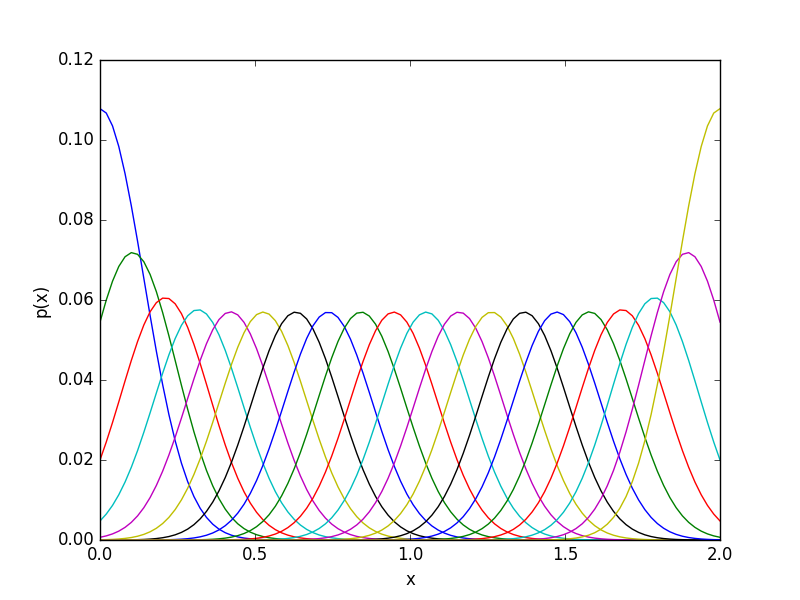
\includegraphics[width=1.0\linewidth]{img/31b}\label{fig:gaussians}

\lstinputlisting[language=Python, firstline = 0]{../Code/31b.py}

\end{answer}

\end{question}

%----------------------------------------------

\begin{question}{Gaussian Features, Continued}{6}
Repeat the process of fitting the model using the Gaussian features from the previous question. Compare the RMSE on the testing data using $15 \ldots 40$ basis functions and plot the RMSE. Which number of basis functions has the best performance and what is the best RMSE? Use a Ridge coefficient of $\lambda=10^{-6}$.

\begin{answer}\end{answer}

\end{question}

%----------------------------------------------

\begin{question}{Bayesian Linear Regression}{10}
Using Bayesian linear regression and polynomial features of 12th degree, plot the mean and the standard deviation of the predictive distribution for each case, using the first $N={10, 12, 16, 20, 50, 150}$ data points.
Discuss how the model uncertainty change with the amount of data points and the problem of overfitting with Bayesian linear regression. Use a prior $\sigma^2=0.0025$.

\begin{answer}\end{answer}
\end{question}

%----------------------------------------------

\begin{question}{Bayesian Linear Regression, Continued}{5}
How can we further reduce the uncertainty? Is it always a good practice?

\begin{answer}\end{answer}
\end{question}

%----------------------------------------------

\begin{question}[bonus]{Cross Validation}{5}
So far, we have split our dataset in two sets: training data and testing data. Cross-validation is a more sophisticated approach for model selection. Discuss it and its variants, pointing out their pro and cons.
\end{question}

\begin{answer}\end{answer}

\end{questions}
